\newpage
\hypertarget{subsec:IndexToLevel}{}
\subsection{Implementing IndexToLevel}
\genHeader

If everything has been done correctly up to this point, your project should save and build without errors in Eclipse. In fact, there should now be three
generated repository projects included in \texttt{MyWorkingSet}. We're most concerned with \texttt{LearningBox\-To\-Dictionary\-Integration}, which implements
our TGG and its rules. Expand your folder so it resembles Fig.~\ref{eclipse:tggGenerated}

\begin{figure}[htbp]
\begin{center}
  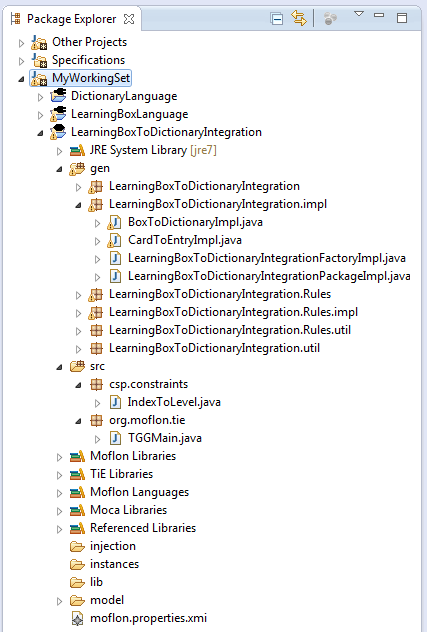
\includegraphics[width=0.7\textwidth]{eclipse_generatedTGG}
  \caption{Files generated from your TGG}
  \label{eclipse:tggGenerated}
\end{center}
\end{figure}

Despite all these files, the TGG isn't yet complete. While we've declared and used our custom \texttt{IndexTolevel} attribute constraint, we haven't actually
implemented it yet. Let's quickly review the purpose of constraints before we do.

\newpage

Just like patterns describing \emph{structural} correspondence, \emph{attribute constraints} can be automatically \emph{operationalized} as required for the
forward concrete transformations. Even more interesting, a set of constraints might have to be ordered in a specific way depending on the direction of the
transformation, or they might have to be checked for pre-existing attributes. Others still might have to set values appropriately in order to fulfill the
constraint.

For built-in \emph{library} constraints such as \emph{eq}, \emph{addPrefix} and \emph{concat}, you do not need to worry about these details and can just focus
on expressing what should happen. Everything else is handled automatically.

In many cases however, a required constraint might be extremely narrow and problem-specific, such as our \emph{IndexToLevel}. There might not be any fitting
combination of library constraints to express the consistency condition, so a new attribute constraint type must be declared before its use.

There is a list of \emph{adornments} in the declaration which specify the cases for which the constraint can be operationalized. Each adornment consists of a
\texttt{B} (bound) or \texttt{F} (free) variable setting for each argument of the constraint. It sounds complex, but is really quite simple, especially in the
context of our example:

\begin{description}

\item[BB] indicates that the \texttt{partition.index} and \texttt{entry.level} are both \emph{bound}, i.e., they already have assigned values.
In this case, the \emph{operation} must check if the assigned values are valid and correct.

\item[BF] indicates that \texttt{partition.index} is \emph{bound} and \texttt{entry.level} is \emph{free}, i.e., the operation must determine and assign the
correct value to \texttt{entry.level} using \texttt{partition.index}.

\item[FB] indicates that \texttt{partition.index} is \emph{free} and \texttt{entry.level} is \emph{bound}, i.e., the operation must determine and assign the
correct value to \texttt{parti\-tion.in\-dex} using \texttt{entry.level}.

\end{description}

Note that we decide not to support \textbf{FF} as we would have to generate a consistent pair of \texttt{index} and \texttt{level}. Although this is possible
and might even make sense for some applications, it does not in the context of partitions and entries (the pairs are not unique, so which pair should we take?
\texttt{partition2} set to \texttt{beginner}?).

At compile time, the set of constraints (also called \emph{Constraint Satisfaction Problem} (CSP)) for every TGG rule is ``solved'' for each case by
operationalizing all constraints and determining a feasible sequence in which the operations can be executed, compatible to the declared adornments of each
constraint. If the CSP cannot be solved, an exception is thrown at compile time

Now that we have a better understanding behind the construction of attribute constraints, let's implement \texttt{IndexToLevel}.

\begin{itemize}
\item[$\blacktriangleright$] Locate and open \texttt{IndexToLevel.java} under ``src/csp.constraints'' in \texttt{LearningBoxToDictionaryIntegration}.

\item[$\blacktriangleright$] As you can see, code has been generated in order to handle the current unimplemented state of \texttt{IndexToLevel}. Use the
Eclipse's built-in auto-complete feature to help implement the code in Fig.~\ref{code:indexToLevel} and replace the default code.\footnote{Although tempting, we
recommend not to copy and paste the contents from your pdf viewer into Eclipse. Invisible characters are likely to be added, and your code might not work.}

\begin{figure}[htbp]
\begin{center}
\begin{lstlisting}[language=Java,backgroundcolor=\color{white}, keywordstyle={\bfseries\color{purple}}]
package csp.constraints;

import java.util.Arrays;
import java.util.List;
import TGGLanguage.csp.Variable;
import TGGLanguage.csp.impl.ConstraintImpl;

public class IndexToLevel extends TGGConstraintImpl {

	private List<String> levels = Arrays.asList(new String[] { "master",
			"advanced", "beginner" });

	public void solve(Variable<Number> var_0, Variable<String> var_1) {

		String bindingStates = getBindingStates(var_0, var_1);
		
		int index = var_0.getValue().intValue();
		String level = var_1.getValue();

		switch (bindingStates) {
		case "BB":
			setSatisfied(levels.get(index).equals(level));
			break;

		case "BF":
			if (index < 0)
				var_1.setValue(levels.get(0));
			else if (index > 2)
				var_1.setValue(levels.get(2));
			else
				var_1.setValue(levels.get(index));

			var_1.setBound(true);
			setSatisfied(true);
			break;

		case "FB":
			index = levels.indexOf(level);
			if (index == -1) {
				setSatisfied(false);
			} else {
				var_0.setValue(index);
				var_0.setBound(true);
				setSatisfied(true);
			}
			break;
		}
	}
}
\end{lstlisting}
  \caption{Implementation of our custom \texttt{IndexToLevel} constraint}
  \label{code:indexToLevel}
\end{center}
\end{figure}

\end{itemize}

To briefly explain, the \texttt{levels} list contains each \texttt{level} at position 0, 1, or 2 in the list, which correspond to our three
\texttt{Partition.index} attributes. You'll notice that instead of setting `master' to 2, it has been set to match the first 0 partition. Unlike an
\texttt{entry} in \texttt{dictionary}, the position of each \texttt{card} in \texttt{box} is \emph{not} based on difficulty, but simply how it has been moved
as a result of the user's guess. Easy cards are more likely to be in the final partition (due to moving through the box quickly) while challenging cards are
most likely to have been returned to the starting position.

In the \texttt{solve} method, there is a switch statement based on whichever adornment is currently active. For all cases, \texttt{setSatisfied}
informs the TGG whether or not the constraint (and by consequence, the precondition of the rule) can be satisfied. For \texttt{BF}, it suggests that if a
negative partition were to exist, to simply set its index value to 0. Similarily, if there was ever a partition more than 2 (i.e., \texttt{partition4}), it
would set its index to the highest difficulty level, 2. Otherwise, \texttt{BF} simply gets the index of the partition, assigns it so it becomes bound, and
terminates. In the final case, where \texttt{level} is already known (i.e., transforming an \texttt{entry} into a \texttt{card}), if the String \texttt{level}
cannot be matched to any of those in the list, the constraint cannot be fulfilled, and the rule cannot be completed.
